% Created by tikzDevice version 0.10.1 on 2016-08-26 10:12:42
% !TEX encoding = UTF-8 Unicode
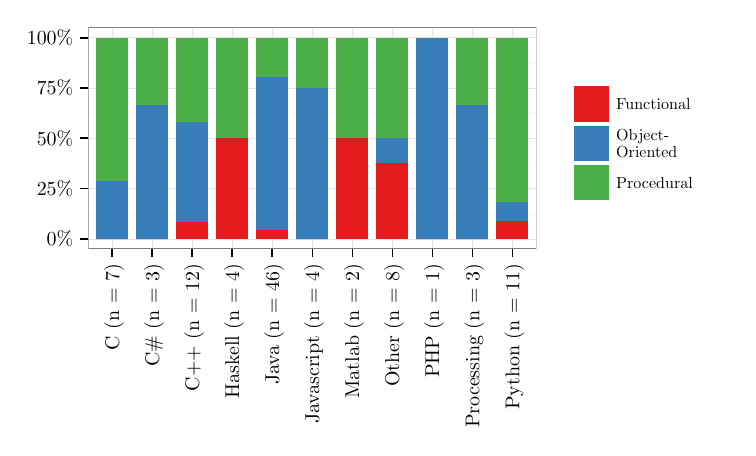
\begin{tikzpicture}[x=1pt,y=1pt]
\definecolor{fillColor}{RGB}{255,255,255}
\path[use as bounding box,fill=fillColor,fill opacity=0.00] (0,0) rectangle (252.94,144.54);
\begin{scope}
\path[clip] (  0.00,  0.00) rectangle (252.94,144.54);
\definecolor{drawColor}{RGB}{255,255,255}
\definecolor{fillColor}{RGB}{255,255,255}

\path[draw=drawColor,line width= 0.6pt,line join=round,line cap=round,fill=fillColor] (  0.00,  0.00) rectangle (252.94,144.54);
\end{scope}
\begin{scope}
\path[clip] ( 21.89, 64.59) rectangle (183.84,144.54);
\definecolor{fillColor}{RGB}{255,255,255}

\path[fill=fillColor] ( 21.89, 64.59) rectangle (183.84,144.54);
\definecolor{drawColor}{gray}{0.98}

\path[draw=drawColor,line width= 0.6pt,line join=round] ( 21.89, 77.31) --
	(183.84, 77.31);

\path[draw=drawColor,line width= 0.6pt,line join=round] ( 21.89, 95.48) --
	(183.84, 95.48);

\path[draw=drawColor,line width= 0.6pt,line join=round] ( 21.89,113.65) --
	(183.84,113.65);

\path[draw=drawColor,line width= 0.6pt,line join=round] ( 21.89,131.82) --
	(183.84,131.82);
\definecolor{drawColor}{gray}{0.90}

\path[draw=drawColor,line width= 0.2pt,line join=round] ( 21.89, 68.22) --
	(183.84, 68.22);

\path[draw=drawColor,line width= 0.2pt,line join=round] ( 21.89, 86.39) --
	(183.84, 86.39);

\path[draw=drawColor,line width= 0.2pt,line join=round] ( 21.89,104.56) --
	(183.84,104.56);

\path[draw=drawColor,line width= 0.2pt,line join=round] ( 21.89,122.73) --
	(183.84,122.73);

\path[draw=drawColor,line width= 0.2pt,line join=round] ( 21.89,140.91) --
	(183.84,140.91);

\path[draw=drawColor,line width= 0.2pt,line join=round] ( 30.56, 64.59) --
	( 30.56,144.54);

\path[draw=drawColor,line width= 0.2pt,line join=round] ( 45.02, 64.59) --
	( 45.02,144.54);

\path[draw=drawColor,line width= 0.2pt,line join=round] ( 59.48, 64.59) --
	( 59.48,144.54);

\path[draw=drawColor,line width= 0.2pt,line join=round] ( 73.94, 64.59) --
	( 73.94,144.54);

\path[draw=drawColor,line width= 0.2pt,line join=round] ( 88.40, 64.59) --
	( 88.40,144.54);

\path[draw=drawColor,line width= 0.2pt,line join=round] (102.86, 64.59) --
	(102.86,144.54);

\path[draw=drawColor,line width= 0.2pt,line join=round] (117.32, 64.59) --
	(117.32,144.54);

\path[draw=drawColor,line width= 0.2pt,line join=round] (131.78, 64.59) --
	(131.78,144.54);

\path[draw=drawColor,line width= 0.2pt,line join=round] (146.24, 64.59) --
	(146.24,144.54);

\path[draw=drawColor,line width= 0.2pt,line join=round] (160.70, 64.59) --
	(160.70,144.54);

\path[draw=drawColor,line width= 0.2pt,line join=round] (175.16, 64.59) --
	(175.16,144.54);
\definecolor{fillColor}{RGB}{228,26,28}

\path[fill=fillColor] ( 24.78, 68.22) rectangle ( 36.35, 68.22);
\definecolor{fillColor}{RGB}{55,126,184}

\path[fill=fillColor] ( 24.78, 68.22) rectangle ( 36.35, 88.99);
\definecolor{fillColor}{RGB}{77,175,74}

\path[fill=fillColor] ( 24.78, 88.99) rectangle ( 36.35,140.91);
\definecolor{fillColor}{RGB}{228,26,28}

\path[fill=fillColor] ( 39.24, 68.22) rectangle ( 50.81, 68.22);
\definecolor{fillColor}{RGB}{55,126,184}

\path[fill=fillColor] ( 39.24, 68.22) rectangle ( 50.81,116.68);
\definecolor{fillColor}{RGB}{77,175,74}

\path[fill=fillColor] ( 39.24,116.68) rectangle ( 50.81,140.91);
\definecolor{fillColor}{RGB}{228,26,28}

\path[fill=fillColor] ( 53.70, 68.22) rectangle ( 65.27, 74.28);
\definecolor{fillColor}{RGB}{55,126,184}

\path[fill=fillColor] ( 53.70, 74.28) rectangle ( 65.27,110.62);
\definecolor{fillColor}{RGB}{77,175,74}

\path[fill=fillColor] ( 53.70,110.62) rectangle ( 65.27,140.91);
\definecolor{fillColor}{RGB}{228,26,28}

\path[fill=fillColor] ( 68.16, 68.22) rectangle ( 79.73,104.56);
\definecolor{fillColor}{RGB}{55,126,184}

\path[fill=fillColor] ( 68.16,104.56) rectangle ( 79.73,104.56);
\definecolor{fillColor}{RGB}{77,175,74}

\path[fill=fillColor] ( 68.16,104.56) rectangle ( 79.73,140.91);
\definecolor{fillColor}{RGB}{228,26,28}

\path[fill=fillColor] ( 82.62, 68.22) rectangle ( 94.19, 71.38);
\definecolor{fillColor}{RGB}{55,126,184}

\path[fill=fillColor] ( 82.62, 71.38) rectangle ( 94.19,126.68);
\definecolor{fillColor}{RGB}{77,175,74}

\path[fill=fillColor] ( 82.62,126.68) rectangle ( 94.19,140.91);
\definecolor{fillColor}{RGB}{228,26,28}

\path[fill=fillColor] ( 97.08, 68.22) rectangle (108.65, 68.22);
\definecolor{fillColor}{RGB}{55,126,184}

\path[fill=fillColor] ( 97.08, 68.22) rectangle (108.65,122.73);
\definecolor{fillColor}{RGB}{77,175,74}

\path[fill=fillColor] ( 97.08,122.73) rectangle (108.65,140.91);
\definecolor{fillColor}{RGB}{228,26,28}

\path[fill=fillColor] (111.54, 68.22) rectangle (123.11,104.56);
\definecolor{fillColor}{RGB}{55,126,184}

\path[fill=fillColor] (111.54,104.56) rectangle (123.11,104.56);
\definecolor{fillColor}{RGB}{77,175,74}

\path[fill=fillColor] (111.54,104.56) rectangle (123.11,140.91);
\definecolor{fillColor}{RGB}{228,26,28}

\path[fill=fillColor] (126.00, 68.22) rectangle (137.57, 95.48);
\definecolor{fillColor}{RGB}{55,126,184}

\path[fill=fillColor] (126.00, 95.48) rectangle (137.57,104.56);
\definecolor{fillColor}{RGB}{77,175,74}

\path[fill=fillColor] (126.00,104.56) rectangle (137.57,140.91);
\definecolor{fillColor}{RGB}{228,26,28}

\path[fill=fillColor] (140.46, 68.22) rectangle (152.03, 68.22);
\definecolor{fillColor}{RGB}{55,126,184}

\path[fill=fillColor] (140.46, 68.22) rectangle (152.03,140.91);
\definecolor{fillColor}{RGB}{77,175,74}

\path[fill=fillColor] (140.46,140.91) rectangle (152.03,140.91);
\definecolor{fillColor}{RGB}{228,26,28}

\path[fill=fillColor] (154.92, 68.22) rectangle (166.49, 68.22);
\definecolor{fillColor}{RGB}{55,126,184}

\path[fill=fillColor] (154.92, 68.22) rectangle (166.49,116.68);
\definecolor{fillColor}{RGB}{77,175,74}

\path[fill=fillColor] (154.92,116.68) rectangle (166.49,140.91);
\definecolor{fillColor}{RGB}{228,26,28}

\path[fill=fillColor] (169.38, 68.22) rectangle (180.95, 74.83);
\definecolor{fillColor}{RGB}{55,126,184}

\path[fill=fillColor] (169.38, 74.83) rectangle (180.95, 81.44);
\definecolor{fillColor}{RGB}{77,175,74}

\path[fill=fillColor] (169.38, 81.44) rectangle (180.95,140.91);
\definecolor{drawColor}{gray}{0.50}

\path[draw=drawColor,line width= 0.6pt,line join=round,line cap=round] ( 21.89, 64.59) rectangle (183.84,144.54);
\end{scope}
\begin{scope}
\path[clip] (  0.00,  0.00) rectangle (252.94,144.54);
\definecolor{drawColor}{RGB}{0,0,0}

\node[text=drawColor,anchor=base east,inner sep=0pt, outer sep=0pt, scale=  0.72] at ( 16.49, 65.74) {0\%};

\node[text=drawColor,anchor=base east,inner sep=0pt, outer sep=0pt, scale=  0.72] at ( 16.49, 83.91) {25\%};

\node[text=drawColor,anchor=base east,inner sep=0pt, outer sep=0pt, scale=  0.72] at ( 16.49,102.08) {50\%};

\node[text=drawColor,anchor=base east,inner sep=0pt, outer sep=0pt, scale=  0.72] at ( 16.49,120.25) {75\%};

\node[text=drawColor,anchor=base east,inner sep=0pt, outer sep=0pt, scale=  0.72] at ( 16.49,138.43) {100\%};
\end{scope}
\begin{scope}
\path[clip] (  0.00,  0.00) rectangle (252.94,144.54);
\definecolor{drawColor}{RGB}{0,0,0}

\path[draw=drawColor,line width= 0.6pt,line join=round] ( 18.89, 68.22) --
	( 21.89, 68.22);

\path[draw=drawColor,line width= 0.6pt,line join=round] ( 18.89, 86.39) --
	( 21.89, 86.39);

\path[draw=drawColor,line width= 0.6pt,line join=round] ( 18.89,104.56) --
	( 21.89,104.56);

\path[draw=drawColor,line width= 0.6pt,line join=round] ( 18.89,122.73) --
	( 21.89,122.73);

\path[draw=drawColor,line width= 0.6pt,line join=round] ( 18.89,140.91) --
	( 21.89,140.91);
\end{scope}
\begin{scope}
\path[clip] (  0.00,  0.00) rectangle (252.94,144.54);
\definecolor{drawColor}{RGB}{0,0,0}

\path[draw=drawColor,line width= 0.6pt,line join=round] ( 30.56, 61.59) --
	( 30.56, 64.59);

\path[draw=drawColor,line width= 0.6pt,line join=round] ( 45.02, 61.59) --
	( 45.02, 64.59);

\path[draw=drawColor,line width= 0.6pt,line join=round] ( 59.48, 61.59) --
	( 59.48, 64.59);

\path[draw=drawColor,line width= 0.6pt,line join=round] ( 73.94, 61.59) --
	( 73.94, 64.59);

\path[draw=drawColor,line width= 0.6pt,line join=round] ( 88.40, 61.59) --
	( 88.40, 64.59);

\path[draw=drawColor,line width= 0.6pt,line join=round] (102.86, 61.59) --
	(102.86, 64.59);

\path[draw=drawColor,line width= 0.6pt,line join=round] (117.32, 61.59) --
	(117.32, 64.59);

\path[draw=drawColor,line width= 0.6pt,line join=round] (131.78, 61.59) --
	(131.78, 64.59);

\path[draw=drawColor,line width= 0.6pt,line join=round] (146.24, 61.59) --
	(146.24, 64.59);

\path[draw=drawColor,line width= 0.6pt,line join=round] (160.70, 61.59) --
	(160.70, 64.59);

\path[draw=drawColor,line width= 0.6pt,line join=round] (175.16, 61.59) --
	(175.16, 64.59);
\end{scope}
\begin{scope}
\path[clip] (  0.00,  0.00) rectangle (252.94,144.54);
\definecolor{drawColor}{RGB}{0,0,0}

\node[text=drawColor,rotate= 90.00,anchor=base east,inner sep=0pt, outer sep=0pt, scale=  0.72] at ( 33.04, 59.19) {C (n = 7)};

\node[text=drawColor,rotate= 90.00,anchor=base east,inner sep=0pt, outer sep=0pt, scale=  0.72] at ( 47.50, 59.19) {C\# (n = 3)};

\node[text=drawColor,rotate= 90.00,anchor=base east,inner sep=0pt, outer sep=0pt, scale=  0.72] at ( 61.96, 59.19) {C++ (n = 12)};

\node[text=drawColor,rotate= 90.00,anchor=base east,inner sep=0pt, outer sep=0pt, scale=  0.72] at ( 76.42, 59.19) {Haskell (n = 4)};

\node[text=drawColor,rotate= 90.00,anchor=base east,inner sep=0pt, outer sep=0pt, scale=  0.72] at ( 90.88, 59.19) {Java (n = 46)};

\node[text=drawColor,rotate= 90.00,anchor=base east,inner sep=0pt, outer sep=0pt, scale=  0.72] at (105.34, 59.19) {Javascript (n = 4)};

\node[text=drawColor,rotate= 90.00,anchor=base east,inner sep=0pt, outer sep=0pt, scale=  0.72] at (119.80, 59.19) {Matlab (n = 2)};

\node[text=drawColor,rotate= 90.00,anchor=base east,inner sep=0pt, outer sep=0pt, scale=  0.72] at (134.26, 59.19) {Other (n = 8)};

\node[text=drawColor,rotate= 90.00,anchor=base east,inner sep=0pt, outer sep=0pt, scale=  0.72] at (148.72, 59.19) {PHP (n = 1)};

\node[text=drawColor,rotate= 90.00,anchor=base east,inner sep=0pt, outer sep=0pt, scale=  0.72] at (163.18, 59.19) {Processing (n = 3)};

\node[text=drawColor,rotate= 90.00,anchor=base east,inner sep=0pt, outer sep=0pt, scale=  0.72] at (177.64, 59.19) {Python (n = 11)};
\end{scope}
\begin{scope}
\path[clip] (  0.00,  0.00) rectangle (252.94,144.54);
\definecolor{fillColor}{RGB}{255,255,255}

\path[fill=fillColor] (192.37, 77.15) rectangle (244.41,131.98);
\end{scope}
\begin{scope}
\path[clip] (  0.00,  0.00) rectangle (252.94,144.54);
\definecolor{fillColor}{RGB}{228,26,28}

\path[fill=fillColor] (197.35,110.58) rectangle (210.16,123.38);
\end{scope}
\begin{scope}
\path[clip] (  0.00,  0.00) rectangle (252.94,144.54);
\definecolor{fillColor}{RGB}{55,126,184}

\path[fill=fillColor] (197.35, 96.35) rectangle (210.16,109.16);
\end{scope}
\begin{scope}
\path[clip] (  0.00,  0.00) rectangle (252.94,144.54);
\definecolor{fillColor}{RGB}{77,175,74}

\path[fill=fillColor] (197.35, 82.13) rectangle (210.16, 94.93);
\end{scope}
\begin{scope}
\path[clip] (  0.00,  0.00) rectangle (252.94,144.54);
\definecolor{drawColor}{RGB}{0,0,0}

\node[text=drawColor,anchor=base west,inner sep=0pt, outer sep=0pt, scale=  0.58] at (212.68,115.00) {Functional};
\end{scope}
\begin{scope}
\path[clip] (  0.00,  0.00) rectangle (252.94,144.54);
\definecolor{drawColor}{RGB}{0,0,0}

\node[text=drawColor,anchor=base west,inner sep=0pt, outer sep=0pt, scale=  0.58] at (212.68,103.88) {Object-};

\node[text=drawColor,anchor=base west,inner sep=0pt, outer sep=0pt, scale=  0.58] at (212.68, 97.66) {Oriented};
\end{scope}
\begin{scope}
\path[clip] (  0.00,  0.00) rectangle (252.94,144.54);
\definecolor{drawColor}{RGB}{0,0,0}

\node[text=drawColor,anchor=base west,inner sep=0pt, outer sep=0pt, scale=  0.58] at (212.68, 86.55) {Procedural};
\end{scope}
\end{tikzpicture}
